%
% 11-gebiete.tex
%
% (c) 2023 Prof Dr Andreas Müller
%

%
% Gebiete
%
\subsection{Gebiete}
Variationsprobleme für Funktionen von nur einer Variablen sind auf 
Funktionen auf einem Intervall beschränkt.
Besteht der Definitionsbereich aus mehreren Intervallen, kann jedes
einzelne Intervall unabhängig von allen anderen betrachtet werden.
Für ein Intervall $[x_0,x_1]$ ist auch das Integral einfach zu definieren,
wie es zur Konstruktion des zu minimierenden Funktionals nötig ist.

Für Funktionen von zwei oder mehr Variablen ist bereits die
Festlegung des Definitionsgebietes viel komplizierter.
Sie muss so erfolgen, dass auch die partielle Integration eines
Produktes darauf übertragbar ist.
Diese wurde im eindimensionalen Fall dazu aus dem Integral
über $F\cdot\eta'$ eine Integral über $dF/dx\cdot \eta$ zu
machen, auf welches das Fundamentallemma anwendbar war.

%
% Offene Mengen
%
\subsubsection{Offene Mengen}
Die Ableitung einer Funktion $f$ in einem Punkt $x\in\mathbb{R}$ erfordert,
dass man Funktionswerte in $x$ mit Funktionswerten in Punkten $x+h$
vergleichen kann, wobei $h\in\mathbb{R}^n$ ein beliebiger kleiner Vektor
sein kann.
Die Ableitung einer Funktion ist dann definiert als die lineare
Ersatzfunktion $Df(x)$ mit der Eigenschaft
\[
f(x+h) = f(x) + Df(x)\cdot h + o(h).
\]
Die Ableitung kann also nur dann sinnvoll definiert werden, wenn
Funktion nicht nur im Punkt $x$, sondern auch in einer Umgebung
des Punktes $x$.
Die Ableitung einer Funktion ist daher nur definiert auf einer
offenen Menge im Sinne der folgenden Definition.
%
% offen.tex
%
% (c) 2024 Prof Dr Andreas Müller
%
\begin{figure}
\centering
%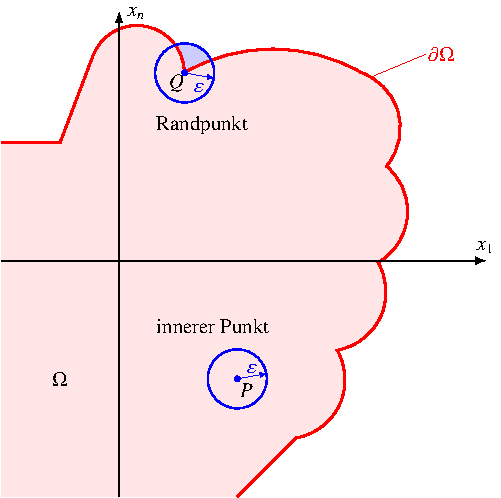
\includegraphics{chapters/040-felder/images/offen.pdf}
\caption{Jeder Punkt einer offenen Menge $\Omega$ besitzt eine kleine
Umgebung, die ebenfalls in der Menge enthalten ist.
Punkte, deren Umgebungen immer Punkte von $\Omega$ und Punkte des
Komplementes $\mathbb{R}^n\setminus\Omega$ enhalten, liegen auf dem
Rand $\partial\Omega$ von $\Omega$.
\label{buch:felder:fundamentallemma:fig:offen}}
\end{figure}


\begin{definition}[offene Menge, Gebiet]
Eine Teilmenge $\Omega\subset\mathbb{R}^n$ heisst {\em offen}, wenn es für
\index{offen}%
jeden Punkt $x\in\Omega$ eine $r>0$ gibt derart, dass ein
Ball mit Radius $r$ um den Punkt $x$ ebenfalls in $\Omega$ enthalten
ist:
\[
B_r(x)
=
\{y\in\mathbb{R}^n
\mid
|y-x|<r\}
\subset \Omega.
\]
Eine offene Menge $\Omega\subset\mathbb{R}$ heisst auch ein {\em Gebiet}.
\index{Gebiet}%
\end{definition}

%
% Der Rand eines Gebietes
%
\subsubsection{Der Rand eines Gebiets}
Die partielle Integration einer Funktion einer Variablen liefert
neben dem Integralterm auch einen Term, der nur von den Werten der
Funktionen an den Endpunkten des Intervalls abhängt.
Es ist zu erwarten, dass ein ähnliches Prinzip auch für die
Integration von Funktionen mehrere Variablen gilt.
Dazu ist jedoch nötig zu erklären, wie genau der Rand eines
Gebietes zu finden ist.

Der Rand eines Intervalls ist einfach zu finden.
Ein Endpunkt eines Intervalls hat die Eigenschaft, dass sich
auf der einen Seite des Punktes lauter Werte befinden, die zum
Intervall gehören, während auf der anderen Seite nur Werte liegen,
die nicht zum Intervall gehören.
Diese anschauliche Beschreibung appelliert aber an eine Vorstellung
einer Richtung und ist daher nicht direkt übersetzbar.
Sie lässt sich aber noch etwas vereinfachen: ein Endpunkt eines
Intervalls hat beliebig nahe Werte die zum Intervall gehören, und
solche die nicht mehr dazu gehören.
Dies suggeriert die folgende Definition für den Rand eines Gebietes.

\begin{definition}[Rand]
\label{buch:felder:fundamentallemma:def:rand}
Ein Randpunkt eines Gebietes $\Omega\subset\mathbb{R}^n$ ist ein Punkt
$x\in\mathbb{R}^n$ mit der Eigenschaft, dass in jeder noch so kleinen 
Umgebung von $x$ Punkte von $\Omega$ und von $\mathbb{R}^n\setminus\Omega$
liegen.
Ein Randpunkt ist also ein Punkt $x\in\mathbb{R}^n$ mit
\[
B_r(x)\cap \Omega\ne \emptyset
\qquad\text{und}\qquad
B_r(x)\cap (\mathbb{R}^n\setminus \Omega)
\ne \emptyset
\]
für alle $r>0$.
Der Rand $\partial \Omega$ eines Gebietes $\Omega$ ist die Menge
aller Randpunkte von $\Omega$.
\end{definition}

Man beachte, dass ein Gebiet $\Omega$ keine Randpunkte enthält.
Wäre $x$ ein Randpunkt von $\Omega$, dann gibt es einen Radius $r$
derart, dass $B_r(x)\in\Omega$ ist.
Für diesen Radius folgt
\[
B_r(x)\cap (\mathbb{R}^n\setminus\Omega)
=
\emptyset,
\]
im Widerspruch zu Annahme, dass $x$ ein Randpunkt war.
Der Widerspruch zeigt, dass ein Punkt von $\Omega$ kein Randpunkt
sein kann.

Die rein punktmengentopologische 
%
% mandelbrot.tex
%
% (c) 2024 Prof Dr Andreas Müller
%
\begin{figure}
\centering
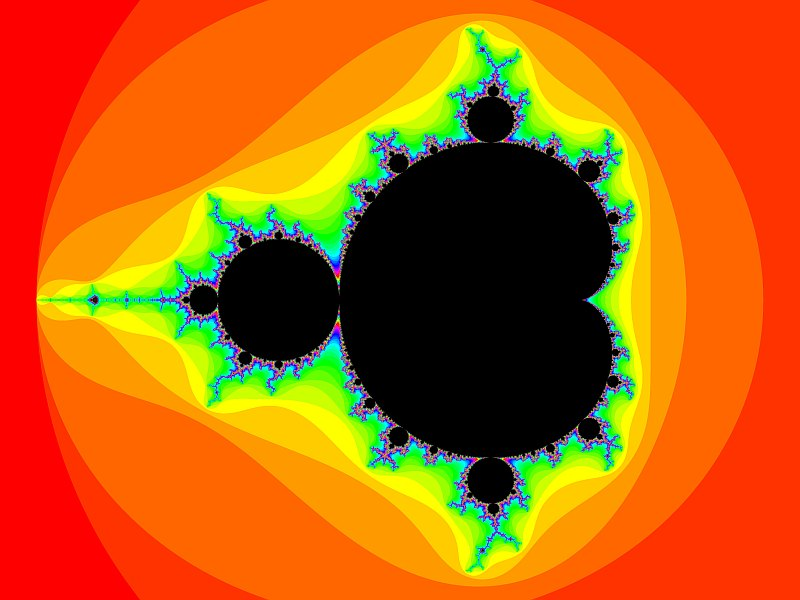
\includegraphics[width=\textwidth]{chapters/040-felder/images/mandelbrot.jpeg}
\caption{Die Mandelbrot-Menge (schwarz) ist berühmt dafür, einen
besonders komplizierten Rand zu haben.
\label{buch:felder:fundamentallemma:fig:mandelbrot}}
\end{figure}
%
Definition~\ref{buch:felder:fundamentallemma:def:rand} des Randes ist
auf Mengen anwendbar, deren Rand sehr kompliziert ist.
Ein Beispiel ist die Mandelbrot-Menge, die in
Abbildung~\ref{buch:felder:fundamentallemma:fig:mandelbrot}
dargestellt ist.
Der schwarze Bereich ist die Mandelbrot-Menge, die farbigen Bereich
liegen ausserhalb der Menge.
Der Rand ist berühmt dafür, dass man beliebig tief hineinzoomen
und immer neue Strukturen entdecken kann.

Im folgenden sollen daher nur solche Gebiete betrachtet werden,
deren Rand die zusätzliche Eigenschaft haben, dass er mit stetigen
oder sogar differenzierbaren Funktionen beschrieben werden kann.
Dies wird von der folgenden Definition erreicht.
%
% randdef.tex
%
\begin{figure}
\centering
%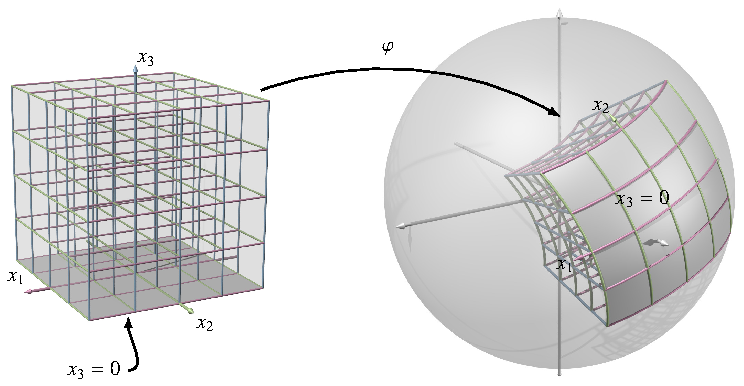
\includegraphics{chapters/040-felder/images/randdef.pdf}
\caption{Der Rand eines Gebietes heisst glatt, wenn jeder Punkt eine
Umgebung hat, die bijektiv und differenzierbar auf eine offene Umgebung
des Nullpunktes abgebildet werden kann, so dass die Hyperebene $x_n=0$
auf den Rand abgebildet wird.
\label{buch:felder:fundamentallemma:fig:randdef}}
\end{figure}


\begin{definition}[glatter Rand]
\label{buch:felder:fundamentallemma:def:glatterrand}
Der Rand eines Gebietes $\Omega\subset\mathbb{R}^n$ heisst {\em glatt},
wenn jeder Punkt $P$ des Randes eine Umgebung hat, in der es eine bijektive
differenzierbare Abbildung
\[
\varphi
\colon
U\to \mathbb{R}^n 
:
x\mapsto \varphi(x)
\]
einer offenen Umgebung $U$ des Nullpunktes gibt derart, dass $\varphi(0)=P$
das Bild $\varphi(x)$ eines Punktes $x=(x_1,\dots,x_{n-1},x_n)$ in $\Omega$
liegt, wenn $x_n\ge 0$ ist, nicht in $\Omega$ liegt, wenn $x_n<0$ ist und auf
dem Rand $\partial\Omega$ liegt, wenn $x_n=0$ ist
(Abbildung~\ref{buch:felder:fundamentallemma:fig:randdef}).
\end{definition}

Ein Gebiet hat also einen glatten Rand, wenn er sich lokal als das
differenzierbare Bild der Hyperebene $x_n=0$ in einer Umgebung des
Nullpunkts in $\mathbb{R}^n$ darstellen lässt.
Für ein beschränktes Gebiet bedeutet dies, dass sich der Rand durch
endlich viele solche Abbildungen parametrisieren lässt.

In zwei Dimensionen kann man den Rand eines Gebietes mit
glattem Rand stückweise als Graphen von differenzierbaren Funktionen
$y_k(x)$ beschreiben, wie dies in
%
% 2drand.tex -- Rand eines zweidmensionalen Gebietes
%
% (c) 2021 Prof Dr Andreas Müller, OST Ostschweizer Fachhochschule
%
\documentclass[tikz]{standalone}
\usepackage{amsmath}
\usepackage{times}
\usepackage{txfonts}
\usepackage{pgfplots}
\usepackage{csvsimple}
\usetikzlibrary{arrows,intersections,math,calc}
\definecolor{darkred}{rgb}{0.8,0,0}
\definecolor{darkgreen}{rgb}{0,0.6,0}
\begin{document}
\def\skala{1}
\begin{tikzpicture}[>=latex,thick,scale=\skala]

\coordinate (P1) at (1,4);
\coordinate (P2) at (7,1);
\coordinate (P3) at (10,2);
\coordinate (P4) at (6,5);
\coordinate (P5) at (9,7);
\coordinate (P6) at (3,7);

\node at (P1) [left] {$P_1$};
%\node at (P2) [below] {$P_2$};
\node at (P3) [right] {$P_2$};
\node at (P4) [right] {$P_3$};
\node at (P5) [right] {$P_4$};
%\node at (P6) [above] {$P_6$};

\fill[color=gray!20]
	(P1)
	to[out=-90,in=180]
	(P2)
	to[out=0,in=-90]
	(P3)
	to[out=90,in=-90]
	(P4)
	to[out=90,in=-90]
	(P5)
	to[out=90,in=0]
	(P6)
	to[out=180,in=90]
	(P1) -- cycle;

\fill[color=blue!10]
	(P1)
	to[out=-90,in=180]
	(P2)
	to[out=0,in=-90]
	(P3)
	-- cycle;
\fill[color=darkred!10]
	(P1)
	--
	(P3)
	to[out=90,in=-90]
	(P4)
	-- cycle;
\fill[color=darkgreen!10]
	(P1)
	--
	(P4)
	to[out=90,in=-90]
	(P5)
	-- cycle;
\fill[color=orange!10]
	(P1)
	--
	(P5)
	to[out=90,in=0]
	(P6)
	to[out=180,in=90]
	(P1) -- cycle;

\draw[line width=0.3pt] (P1) -- (P3);
\draw[line width=0.3pt] (P1) -- (P4);
\draw[line width=0.3pt] (P1) -- (P5);

\draw[color=blue,line width=1.4pt]
	(P1)
	to[out=-90,in=180]
	(P2)
	to[out=0,in=-90]
	(P3);
\draw[color=darkred,line width=1.4pt]
	(P3)
	to[out=90,in=-90]
	(P4);
\draw[color=darkgreen,line width=1.4pt]
	(P4)
	to[out=90,in=-90]
	(P5);
\draw[color=orange,line width=1.4pt]
	(P5)
	to[out=90,in=0]
	(P6)
	to[out=180,in=90]
	(P1);

\fill[color=white] (P1) circle[radius=0.05];
%\fill[color=white] (P2) circle[radius=0.05];
\fill[color=white] (P3) circle[radius=0.05];
\fill[color=white] (P4) circle[radius=0.05];
\fill[color=white] (P5) circle[radius=0.05];
%\fill[color=white] (P6) circle[radius=0.05];

\draw (P1) circle[radius=0.05];
%\draw (P2) circle[radius=0.05];
\draw (P3) circle[radius=0.05];
\draw (P4) circle[radius=0.05];
\draw (P5) circle[radius=0.05];
%\draw (P6) circle[radius=0.05];

\node[color=blue]      at (P2) [below]                  {$y_{12}(x)$};
\node[color=darkred]   at ($0.5*(P3)+0.5*(P4)$) [above] {$y_{23}(x)$};
\node[color=darkgreen] at ($0.5*(P4)+0.5*(P5)$) [below] {$y_{34}(x)$};
\node[color=orange]    at (P6) [above]                  {$y_{41}(x)$};

\draw[->] (0,-0.1) -- (0,8.3) coordinate[label={right:$y$}];
\draw[->] (-0.1,0) -- (11.3,0) coordinate[label={$x$}];

\end{tikzpicture}
\end{document}


Abbildung~\ref{buch:felder:fundamentallemma:fig:2drand}
dargestellt ist.
Mit dieser Definition lassen sich aber natürlich vorkommende Gebiete
wie ein Rechteck $(x_1,x_2)\times(y_1,y_2)$ nicht beschreiben, da
es in den Ecken des Rechtecks keine Abbildung gibt, wie sie in der
Definition~\ref{buch:felder:fundamentallemma:def:glatterrand}
verlangt wird.

%
% Integration über ein Gebiet
%
\subsubsection{Integration über ein Gebiet}
Eine Variationsaufgabe sucht eine Funktion, die ein Integral minimiert,
dessen Integrand von der Funktion abhängt.
Im Falle einer Funktion einer Variablen ist das Definitionsgebiet der
Funktion ein Intervall $I=[x_0,x_1]$, die Funktion $y\colon I\to\mathbb{R}$
wird als differenzierbar angenommen und das zu minimierende Funktional
ist
\[
J(y)
=
\int_{x_0}^{x_1} L(x,y(x),y'(x))\,dx
=
\int_I L(x,y(x),y'(x))\,dx.
\]
Für Funktionen mehrerer Variablen muss also insbesondere der Begriff
der Integration auf ein Integral über ein Gebiet verallgemeinert werden.

Eine Funktion $f(x) = f(x_1,\dots,x_n)$ kann über beliebige
Koordinatenrechtecke oder mehrdimensionale Quader $R$,
die durch Ungleichungen $a_i< x_i<b_i$ gegeben sind, durch das iterierte
Integral
\[
\int_R f(x)
\,dx
=
\int_{a_1}^{b_1}
\dots
\int_{a_n}^{b_n}
f(x_1,\dots,x_n)
\,dx_n
\dots
\,dx_1
\]
berechnet werden.

Das Gebiet $G$ kann durch Quader $R_k$ approximiert werden
(Abbildung~\ref{buch:felder:fig:unterteilung}),
%
% unterteilung.tex -- Unterteilung eines Gebietes
%
% (c) 2021 Prof Dr Andreas Müller, OST Ostschweizer Fachhochschule
%
\documentclass[tikz]{standalone}
\usepackage{amsmath}
\usepackage{times}
\usepackage{txfonts}
\usepackage{pgfplots}
\usepackage{csvsimple}
\usetikzlibrary{arrows,intersections,math}
\definecolor{darkred}{rgb}{0.8,0,0}
\begin{document}
\def\skala{1}
\def\rechteck#1#2#3#4#5#6{
	\fill[color=gray!20]
		({#1*exp(-(#5)*ln(2))},{#2*exp(-(#5)*ln(2))})
		rectangle
		({#3*exp(-(#5)*ln(2))},{#4*exp(-(#5)*ln(2))});
	\draw	({#1*exp(-(#5)*ln(2))},{#2*exp(-(#5)*ln(2))})
		rectangle
		({#3*exp(-(#5)*ln(2))},{#4*exp(-(#5)*ln(2))});
	\node at ({0.5*(#1+#3)*exp(-(#5)*ln(2))},{0.5*(#2+#4)*exp(-(#5)*ln(2))})
		{$#6$};
}
\begin{tikzpicture}[>=latex,thick,scale=\skala]

\coordinate (A) at (1,3);
\coordinate (B) at (7,1);
\coordinate (C) at (6,4);

\fill[color=darkred!20]
	(A)
	to[out=-80,in=-170]
	(B)
	to[out=10,in=-30]
	(C)
	to[out=150,in=100]
	cycle;

\draw[line width=1.4pt,color=darkred]
	(A)
	to[out=-80,in=-170]
	(B)
	to[out=10,in=-30]
	(C)
	to[out=150,in=100]
	cycle;

\node[color=darkred] at (C) [above right] {$G$};

\rechteck{2}{2}{6}{4}{0}{R_0}

\rechteck{4}{3}{6}{4}{1}{R_6}
\rechteck{6}{2}{13}{4}{1}{R_1}
\rechteck{12}{4}{14}{6}{1}{R_2}
\rechteck{12}{6}{13}{7}{1}{}
\rechteck{5}{8}{9}{9}{1}{R_3}
\rechteck{3}{4}{4}{6}{1}{R_5}
\rechteck{2}{6}{4}{7}{1}{R_4}
\rechteck{3}{7}{4}{8}{1}{}
\rechteck{13}{3}{14}{4}{1}{}

\rechteck{26}{5}{29}{6}{2}{}
\rechteck{26}{4}{27}{5}{2}{}
\rechteck{28}{6}{29}{10}{2}{}
\rechteck{26}{12}{27}{13}{2}{}
\rechteck{24}{14}{25}{15}{2}{}
\rechteck{18}{16}{21}{17}{2}{}
\rechteck{7}{16}{10}{17}{2}{}
\rechteck{5}{14}{6}{15}{2}{}
\rechteck{5}{10}{6}{12}{2}{}
\rechteck{7}{7}{8}{8}{2}{}
\rechteck{10}{5}{12}{6}{2}{}

\rechteck{18}{11}{20}{12}{3}{}
\rechteck{19}{10}{20}{11}{3}{}
\rechteck{22}{9}{24}{10}{3}{}
\rechteck{30}{7}{47}{8}{3}{}
\rechteck{54}{8}{55}{10}{3}{}
\rechteck{55}{9}{58}{10}{3}{}
\rechteck{58}{10}{59}{18}{3}{}
\rechteck{56}{20}{57}{22}{3}{}
\rechteck{54}{24}{55}{25}{3}{}
\rechteck{52}{26}{53}{27}{3}{}
\rechteck{50}{28}{51}{29}{3}{}
\rechteck{48}{30}{49}{31}{3}{}
\rechteck{42}{32}{45}{33}{3}{}
\rechteck{42}{33}{43}{34}{3}{}
\rechteck{36}{34}{40}{35}{3}{}
\rechteck{25}{36}{28}{37}{3}{}
\rechteck{19}{34}{20}{36}{3}{}
\rechteck{15}{34}{19}{35}{3}{}
\rechteck{12}{32}{14}{33}{3}{}
\rechteck{13}{33}{14}{34}{3}{}
\rechteck{10}{30}{12}{31}{3}{}
\rechteck{11}{31}{12}{32}{3}{}
\rechteck{9}{28}{10}{30}{3}{}
\rechteck{9}{21}{10}{24}{3}{}
\rechteck{10}{19}{12}{20}{3}{}
\rechteck{11}{17}{12}{19}{3}{}
\rechteck{13}{15}{14}{16}{3}{}
\rechteck{15}{13}{16}{14}{3}{}

\draw[->] (-0.1,0) -- (8.6,0) coordinate[label={$x$}];
\draw[->] (0,-0.1) -- (0,5.6) coordinate[label={right:$y$}];

\end{tikzpicture}
\end{document}


das Integral der Funktion $f$ wird dann durch die Summe
\begin{equation}
\int_G f(x)\,dx
\approx
\sum_k
\int_{R_k} f(x)\,dx
\label{buch:felder:gebiete:eqn:GintegralR}
\end{equation}
approximiert.
Durch Verfeinerung der Quader kann das Gebiet beliebig vollständig überdeckt
werden und damit das Integral beliebig genau approximiert werden.
Der Grenzwert der Summe~\eqref{buch:felder:gebiete:eqn:GintegralR}
ist das Integral der Funktion $f$ über das Gebiet $G$.

%
% Integral über $G$ als iteriertes eindimensionales Integral
%
\subsubsection{Integral über $G$ als iteriertes eindimensionales Integral}
Ein konvexes Gebiet $G$ wie zum Beispiel die Ellipse
\[
G
=
\biggl\{
(x_1,x_2)
\,
\bigg|
\,
\frac{x_1^2}{a^2}+\frac{x_2^2}{b^2}< 1
\biggr\}
\]
kann auch durch die Ungleichungen
\begin{align*}
-b\sqrt{1-\frac{x_1^2}{a^2}}
&< x_2 <
b\sqrt{1-\frac{x_1^2}{a^2}}
&&\text{für $x_1\in (-a,a)$}
\intertext{bzw.}
-a\sqrt{1-\frac{x_2^2}{b^2}}
&< x_1 <
a\sqrt{1-\frac{x_2^2}{b^2}}
&&\text{für $x_2\in (-b,b)$}
\end{align*}
beschrieben werden.
Etwas allgemeiner gibt es Funktionen
$x_{2,\pm}(x_1)$ 
und
$x_{1,\pm}(x_2)$ 
derart, dass das Gebiet $G$ durch die Ungleichungen
\begin{align*}
x_{2,-}(x_1) &< x_2 < x_{2,+}(x_1)&& \text{für $x_1\in(x_{10},x_{11})$}
\intertext{bzw.}
x_{1,-}(x_2) &< x_1 < x_{1,+}(x_2)&& \text{für $x_2\in(x_{20},x_{21})$}
\end{align*}
gegeben ist.
Mit diesen Bezeichnungen lässt sich das Integral über das Gebiet auch
auf zwei verschiedene Arten als das iterierte Integral
\[
\int_G f(x) \,dx
=
\int_{x_{10}}^{x_{11}}
\int_{x_{2,-}(x_1)}^{x_{2,+}(x_1)} f(x_1,x_2)\,dx_2\,dx_1
=
\int_{x_{20}}^{x_{21}}
\int_{x_{1,-}(x_2)}^{x_{1,+}(x_2)} f(x_1,x_2)\,dx_1\,dx_2
\]
geschrieben werden.
Änliche iterierte Integrale können verwenden werden, um Integrale
über Gebiete zu berechnen, deren Dimension grösser als $2$ ist.

Kompliziertere Gebiete, wie die in
Abbildung~\ref{buch:felder:fundamentallemma:fig:2drand}
dargestellten konvexen zweidimensionalen Gebiete, können durch Summen solcher
Integrale berechnet werden.

%
% Integration und Koordinatentransformation
%
\subsubsection{Integration und Koordinatentransformationen}
Unter einer Koordinatentransformation im Definitionsgebiet 
$G$ einer Funktion ändert sich der geometrische Sachverhalt nicht,
das Integral der Funktion sollte sich nicht ändern.
Seien $x_i=x_i(y_1,\dots,y_n)$ Funktionen, die die alten Koordinaten
durch die neuen Koordinaten $y_1,\dots,y_n$ ausdrücken.
Die zusammengesetze Funktion
\[
f(x(y))
=
f(x_1(y_1,\dots,y_n),\dots,x_n(y_1,\dots,y_n))
\]
hat ein Gebiet $\tilde{G}$ als Definitionsgebiet.
Approximiert man $\tilde{G}$ mit Quader $\tilde{R}_k$, dann sind
die Bildmengen $x(\tilde{R}_k)$ keine Quader.
Da die Funktionen $x_i$ differenzierbar, sind sie jedoch näherungsweise
Quader.
Durch die Abbildung $x$ werden die Kantenvektoren $e_j$ der Quader 
$\tilde{R}_k$ auf die Vektoren $Dx\cdot e_j$ abgebildet, die ein
Parallelepiped mit dem Volumen
\[
\det Dx
=
\left|
\renewcommand{\arraystretch}{1.9}
\begin{matrix}
\displaystyle
\frac{\partial x_1}{\partial y_1}
&
\displaystyle
\frac{\partial x_1}{\partial y_2}
&\dots&
\displaystyle
\frac{\partial x_1}{\partial y_n}
\\
\displaystyle
\frac{\partial x_2}{\partial y_1}
&
\displaystyle
\frac{\partial x_2}{\partial y_2}
&\dots&
\displaystyle
\frac{\partial x_2}{\partial y_n}
\\
\vdots&\vdots&\ddots&\vdots\\
\displaystyle
\frac{\partial x_n}{\partial y_1}
&
\displaystyle
\frac{\partial x_n}{\partial y_2}
&\dots&
\displaystyle
\frac{\partial x_n}{\partial y_n}
\end{matrix}
\right|
\]
aufspannen.
Mit dem zusätzlichen Faktor $\det Dx$ kann daher dem Integral einer Funktion
über ein Gebiet eine koordinatensystemunabhängige Bedeutung gegeben werden.

%
% Volumenelement
%
\subsubsection{Volumenelement}
Die Notwendigkeit, bei einer Variablentransformation den Faktor
$\det Dx$ hinzuzufügen, zeigt, dass ein vom Koordinatensystem unabhängiges
Integral einer Funktion über ein Gebiet $G$ erst durch eine zusätzliche
Gewichtsfunktion $g(x)$ definiert ist, die sich beim Wechsel des
Koordinatensystems mit der Determinanten der Ableitung $Dx$ multipliziert.
Die Gewichtsfunktion ist im willkürlich.
Sie wird erst eindeutig,
wenn die Verbindung zwischen dem Volumeninhalt des Gebietes und 
dem Integral dadurch hergestellt wird, dass das Integral der konstanten
Funktion $1$ das Volumen
\[
\operatorname{vol}(G)
=
\int_G 1\cdot g(x)\,dx
\]
sein soll.

Für kartesische Koordinaten ist die diese Gewichtsfunktion $g(x)=1$.
Wählt man stattdessen Kugelkoordinaten $(r,\vartheta,\varphi)$, mit der
Koordinatentransformation
\begin{equation}
\left.
\begin{aligned}
x&=r\sin\vartheta\cos\varphi\\
y&=r\sin\vartheta\sin\varphi\\
z&=r\cos\vartheta
\end{aligned}
\;\right\}
\qquad
\Rightarrow
\qquad
Dx
=
\begin{pmatrix}
\sin\vartheta\cos\varphi
	&  r \cos\vartheta\cos\varphi
		& -r\sin\vartheta\sin\varphi\\
\sin\vartheta\sin\varphi
	&  r \cos\vartheta\sin\varphi
		& \phantom{-}r\sin\vartheta\cos\varphi\\
\cos\vartheta
	& -r \sin\vartheta
		& \phantom{-}0
\end{pmatrix},
\end{equation}
deren Determinante
\begin{align*}
\det Dx
&=
r^2\bigl(
\cos\vartheta
(\cos\vartheta \sin\vartheta \cos^2\varphi
+
\cos\vartheta \sin\vartheta \sin^2\varphi
)
\\
&\phantom{=}
\quad
+
\sin\vartheta
(
\sin^2\vartheta \cos^2\varphi
+
\sin^2\vartheta \sin^2\varphi
)
\bigr)
\\
&=
r^2\bigl(
\cos^2\vartheta\sin\vartheta
+
\sin^3\vartheta
\bigr)
\\
&=
r^2
\sin\vartheta
\bigl(
\cos^2\vartheta
+
\sin^2\vartheta
\bigr)
\\
&=
r^2\sin\vartheta
\end{align*}
ist.
In Kugelkoordinaten ist das Integral daher als
\[
\int_G f(r,\vartheta,\varphi)
\,
r^2\sin^2\varphi
\,dr\,d\vartheta\,d\varphi
\]
zu berechnen.
Die Gewichtsfunktion $g(r,\vartheta,\varphi)=r^2\sin\vartheta$ ergibt
zusammen mit den Differentialen des Integrals das sogenannte
{\em Volumenelement}
\(
r^2\sin\vartheta\,dr\,d\vartheta\,d\varphi
\).
\index{Volumenelement}%

%
% Integration über eine Kurve
%
\subsubsection{Integration über eine Kurve}
Ein besonders einfacher Fall ist das Integral über eine Kurve.
Mit Hilfe einer Parametrisierung $\gamma_1\colon I_1\to\mathbb{R}^n$
einer Kurve wird ein Integral über die Werte einer Funktion $f$, die auf
der Bildmenge $\gamma_1(I_1)$ definiert ist, zu einem Integral
\begin{equation}
\int_{I_1}
f(\gamma_1(t))
\,dt
\label{buch:felder:gebiete:eqn:kurvenintegral}
\end{equation}
der Funktion $f\circ\gamma\colon I_1\to\mathbb{R}:t\mapsto f(\gamma_1(t))$
über ein Intervall der reellen Achse.
Dabei spielt aber offenbar die Parametrisierung eine Rolle.
Eine alternative Parametrisierung $\gamma_2\colon I_2\to\mathbb{R}^n$,
lässt sich immer durch eine Koordinatentransformation $u\colon I_2\to I_1$
in $\gamma_2 = \gamma_1\circ u$ überführen.
Dabei geht das Integral
\eqref{buch:felder:gebiete:eqn:kurvenintegral}
mit der Substitution $t=u(s)$
über in das Integral
\[
\int_{i_1}
f(\gamma_1(t))
\,dt
=
\int_{I_2}
f(\gamma_1(u(s)))
\,
u'(s)
\,ds
=
\int_{I_2}
f(\gamma_2(s))
\,
u'(s)
\,ds.
\]
Der zusätzliche Faktor $u'(s)$ gibt wieder, wie die Umparametrisierung
die Kurvenlänge verzerrt.


%
% Integration über den Rand
%
\subsubsection{Integration über den Rand}


